% Reproducibility sheet template. Filled by scripts/15_build_repro_sheet.py: every double-angle-bracket
% placeholder is computed from artifacts/ and reports/ at build time. Edit the prose here, never the numbers.
\documentclass[11pt]{article}
\usepackage[margin=1in]{geometry}
\usepackage{booktabs,longtable,array,graphicx,fancyvrb,enumitem,caption}
\usepackage{xurl}
\usepackage[hidelinks]{hyperref}
\setlength{\parindent}{0pt}
\setlength{\parskip}{6pt}
\setlength{\emergencystretch}{3em}
\captionsetup{font=small,labelfont=bf,skip=4pt}
\setlength{\LTpre}{6pt}
\setlength{\LTpost}{6pt}
\newcolumntype{P}[1]{>{\raggedright\arraybackslash}p{#1}}

\begin{document}

\begin{center}
{\LARGE\bfseries Reproducibility Sheet}\\[6pt]
{\large Multi-Turn Reinforcement Learning on Amazon SageMaker AI:\\
Training a Customer-Support Agent on GPT-OSS-20B}\\[12pt]
{\large Isham Rashik}\\[4pt]
Run of record: 2026-10-01 23:14 UTC to 2026-10-02 05:29 UTC
\end{center}

This sheet accompanies the workshop notebook \texttt{notebooks/sagemaker\_mtrl\_real\_demo.ipynb} and the
repository's \texttt{README.md}. With it, anyone with a clean copy of the repository can rebuild every table,
figure, and headline number from the recorded evidence without an AWS account, and can repeat the study in
their own AWS account. The interpretation lives in the notebook and the README; what follows is the recipe.
Every step is a numbered script in \texttt{scripts/} that imports the shared \texttt{aws} package, and the
agent that SageMaker trained against is in \texttt{agent/}. This sheet is itself generated by
\texttt{scripts/15\_build\_repro\_sheet.py}: every number below is read from \texttt{artifacts/} and
\texttt{reports/} when the sheet is built, and the build refuses to run unless every invariant passes, so the
sheet cannot drift from the evidence.

\section{Repository and Run Identifiers}
\begin{center}
\begin{minipage}{\linewidth}\centering
\begin{tabular}{P{3.6cm}P{11.8cm}}
\toprule
\textbf{Item} & \textbf{Value} \\
\midrule
Repository commit & not yet under version control \\
AWS account and regions & 384887233198; us-west-2 (SageMaker AI, AgentCore, MLflow, S3), us-east-1 (Bedrock import) \\
Training job & \texttt{openai-reasoning-gpt-oss-20b-mtrl-20261002040558} \\
Model package & \texttt{openai-reasoning-gpt-oss-20b-mtrl-mpg/1} \\
Imported model & \nolinkurl{arn:aws:bedrock:us-east-1:384887233198:imported-model/ffakmfmpoqbi} \\
Official guide & \url{https://docs.aws.amazon.com/sagemaker/latest/dg/model-customize-mtrl.html} \\
\bottomrule
\end{tabular}
\end{minipage}
\end{center}
The commit row fills in automatically once the project is under version control; rebuild this sheet after the first commit.

\section{Hardware and Operating System}
All model computation ran on AWS managed services. The local machine only submits and re-attaches to jobs,
drives the live inference, and builds the reports, so local hardware does not affect any reported number.
\begin{center}
\begin{minipage}{\linewidth}\centering
\begin{tabular}{P{4.6cm}P{10.8cm}}
\toprule
\textbf{Role} & \textbf{Where it ran} \\
\midrule
Run of record (orchestration, live inference, reports) & macOS 26 (Darwin 25.3), Apple silicon (arm64), Python 3.12.10 \\
This build of the sheet & Darwin 25.3.0 (arm64), Python 3.12.10 \\
Training and evaluation & Amazon SageMaker AI multi-turn RL, serverless (instances are managed and not exposed); base model openai-reasoning-gpt-oss-20b/3.43.0 \\
Agent environment & Amazon Bedrock AgentCore Runtime version 7, linux/arm64 container on python:3.12-slim (digests in Section 12.6) \\
Deployment option 1 & SageMaker real-time endpoint on ml.g6e.12xlarge: not provisioned (InsufficientInstanceCapacity); nothing billed \\
Deployment option 2 & Amazon Bedrock Custom Model Import, us-east-1; serverless, billed per active model minute \\
Linux & requirements-linux.txt carries the same direct pins; the pipeline has not been run on Linux \\
\bottomrule
\end{tabular}
\end{minipage}
\end{center}

\section{Software Environment}
The local environment is a conda environment named \texttt{aws-mtrl} (Python 3.12). Three levels of pinning
are committed:
\begin{itemize}[leftmargin=*]
\item \texttt{environment-macos.yaml} and \texttt{requirements-macos.txt}: the direct dependencies at exact
versions (run of record: macOS). \texttt{environment-linux.yaml} and \texttt{requirements-linux.txt} carry the
same pins and have not been verified on Linux.
\item \texttt{requirements-macos.lock.txt}: every installed distribution (259) of the environment
that ran the scripts and the live inference.
\item \texttt{agent/requirements.lock.txt}: the exact 139 packages of the container image that
served every rollout, read from its CodeBuild log, with the base-image digest.
\end{itemize}
\begin{Verbatim}[frame=single,fontsize=\small]
conda env create -f environment-macos.yaml      # or environment-linux.yaml
conda activate aws-mtrl
pip install -r requirements-macos.lock.txt      # optional: the exact full environment
\end{Verbatim}
\begin{center}
\begin{minipage}{\linewidth}\centering
\captionof{table}{Direct dependencies (\texttt{requirements-macos.txt}).}
\begin{tabular}{llll}
\toprule
\textbf{Package} & \textbf{Version} & \textbf{Package} & \textbf{Version} \\
\midrule
python & 3.12.10 & openai & 2.54.0 \\
bedrock-agentcore & 1.24.0 & pandas & 3.0.6 \\
bedrock-agentcore-starter-toolkit & 0.3.13 & pyarrow & 25.0.1 \\
boto3 & 1.43.107 & pydantic & 2.13.5 \\
botocore & 1.43.107 & pytest & 9.1.1 \\
ipykernel & 7.4.0 & requests & 2.34.2 \\
jupyterlab & 4.6.4 & sagemaker & 3.23.0 \\
matplotlib & 3.11.2 & sagemaker-core & 2.23.0 \\
mlflow & 3.16.1 & sagemaker-mlflow & 0.5.0 \\
mypy-boto3-sagemaker-runtime & 1.43.68 & sagemaker-mlops & 1.23.0 \\
nbconvert & 7.17.1 & sagemaker-serve & 1.23.0 \\
nbformat & 5.11.1 & sagemaker-train & 1.23.0 \\
numpy & 2.5.3 & strands-agents & 1.57.2 \\
\bottomrule
\end{tabular}
\end{minipage}
\end{center}

\section{Data}
Two committed prompt files define the study, and nothing is resampled. Training needs more prompts than the
global batch size (32), which is why the training set grew from 32 to 64 tickets before the
training job; the original 32 are kept in \texttt{artifacts/training\_prompts.32.csv}.
{\small
\begin{center}
\begin{minipage}{\linewidth}\centering
\begin{tabular}{lrrl}
\toprule
\textbf{File (in data/)} & \textbf{Rows} & \textbf{Unique} & \textbf{SHA-256} \\
\midrule
\texttt{training\_prompts.csv} & 64 & 64 & \texttt{\scriptsize 1c61077a792df2c7ce19a00f38abe8b96a2bf146abe031c41fd8ab7c6c807277} \\
\texttt{evaluation\_prompts.csv} & 32 & 32 & \texttt{\scriptsize 213538946018bdc334ed3b764ccaf16bee8f9bc9bef514adc5899608221e60cf} \\
\bottomrule
\end{tabular}
\end{minipage}
\end{center}
}
The held-out set never enters training: the two files share no prompt (invariant~2), and both
are byte-identical to the run of record (invariant~3). The CSVs were converted to Parquet
and uploaded to S3 before the jobs ran. \texttt{scripts/11b\_snapshot\_provenance.py} later compared those S3
objects with the CSVs, prompt by prompt, and recorded when they were written
(invariant~4):
{\small
\begin{center}
\begin{minipage}{\linewidth}\centering
\begin{tabular}{lP{4.8cm}P{2.3cm}cP{4.1cm}}
\toprule
\textbf{Split} & \textbf{S3 object (datasets/)} & \textbf{Written} & \textbf{Equals CSV} & \textbf{Read by (start)} \\
\midrule
training & \texttt{training\_prompts.parquet} & 2026-10-02 00:05:39 UTC & yes & Training 2026-10-02 00:05:58 UTC \\
evaluation & \texttt{evaluation\_prompts.parquet} & 2026-10-01 22:37:50 UTC & yes & Base evaluation 2026-10-01 23:14:50 UTC; Comparison evaluation 2026-10-02 00:26:56 UTC \\
\bottomrule
\end{tabular}
\end{minipage}
\end{center}
}

\section{Random Seeds and Sources of Randomness}
\begin{center}
\begin{minipage}{\linewidth}\centering
\begin{tabular}{P{4.6cm}P{3.6cm}P{6.8cm}}
\toprule
\textbf{Purpose} & \textbf{Value} & \textbf{Where set} \\
\midrule
Live inference: action order & 2026 & aws/config.py (inference\_seed); recorded in inference\_before\_after.json \\
Live inference: tickets & first 6 held-out, in file order & aws/config.py (inference\_ticket\_count) \\
Rollout action order (training and evaluation) & random per episode & agent/app.py (secrets.randbits); recorded per rollout as action\_order\_seed \\
SageMaker MTRL sampling and LoRA updates & not seedable & service-side \\
Bedrock sampling (live inference) & not seedable & service-side \\
\bottomrule
\end{tabular}
\end{minipage}
\end{center}
The study is therefore reproducible at two levels. Exactly: the offline steps rebuild every table, figure,
and this sheet from the evidence with identical values. Statistically: a new run uses the same code, data,
settings, and pins, but service-side sampling cannot be seeded, so its numbers differ within sampling noise.
With 64 rollouts per model, pass@1 has a standard error of about 0.052 (fine-tuned) to 0.062 (base). The same base
model scored pass@1 0.500 in the baseline and 0.578 in the comparison, on
the same tickets.

\section{Compute Accounting and Budgets}
Costs are recorded per job and never silently merged. Token-priced lines use the token counts AWS billed
(\texttt{BillableTokenUsage}) at the AWS Price List rates in effect, in USD per million tokens: training prefill 0.12, sample 0.30, train 0.36; evaluation prefill 0.12, sample 0.30.
The other lines are computed or estimated, and their labels say how. AWS Cost Explorer is the final bill.
Each line's token usage is in \texttt{artifacts/cost\_accounting.json}; the table is
\texttt{reports/repro/compute\_accounting.csv}.
\begin{longtable}{P{5.6cm}P{4.4cm}rP{2.6cm}}
\caption{Compute accounting.} \\
\toprule
\textbf{Item} & \textbf{Billed tokens} & \textbf{USD} & \textbf{Source} \\
\midrule
\endfirsthead
\multicolumn{4}{l}{\textit{continued}} \\
\toprule
\textbf{Item} & \textbf{Billed tokens} & \textbf{USD} & \textbf{Source} \\
\midrule
\endhead
\bottomrule
\endlastfoot
Base evaluation (first attempt) & prefill 43,488, sample 5,591 & 0.0069 & billed tokens x rate \\
Base evaluation & prefill 197,217, sample 34,617 & 0.0341 & billed tokens x rate \\
Training & prefill 4,833,702, sample 778,911, train 5,599,613 & 2.8296 & billed tokens x rate \\
Comparison: base model & prefill 212,274, sample 33,573 & 0.0355 & billed tokens x rate \\
Comparison: fine-tuned model & prefill 229,165, sample 28,952 & 0.0362 & billed tokens x rate \\
Cross-region copy of weights to us-east-1 (41.8 GB x \$0.02/GB) & -- & 0.8400 & computed or estimated \\
Bedrock imported model inference (estimate: 1 CMU x \textasciitilde{}35 active min x \$0.0572) & -- & 2.0000 & computed or estimated \\
Endpoint uptime & -- & 0.0000 & computed or estimated \\
Contingency (AgentCore, CodeBuild, S3, logs) & -- & 2.0000 & allowance \\
\end{longtable}
Billed tokens \$2.94 plus computed or estimated \$2.84 gives \$5.78; with the allowance for unmeasured AgentCore, CodeBuild, S3, and logs, \$7.78, against the \$25 hard cap.
\begin{center}
\begin{minipage}{\linewidth}\centering
\begin{tabular}{P{5.2cm}P{4.2cm}P{5.6cm}}
\toprule
\textbf{Job} & \textbf{Started} & \textbf{Duration} \\
\midrule
Base evaluation (of record) & 2026-10-01 23:14:50 UTC & n/c \\
Training (10 steps) & 2026-10-02 00:05:58 UTC & 19.2 min \\
Comparison evaluation & 2026-10-02 00:26:56 UTC & n/c \\
Endpoint attempt (option 1) & 2026-10-02 04:14:34 UTC & 38.4 min until deleted; never InService \\
Bedrock import job (option 2) & 2026-10-02 05:15:33 UTC & 13.8 min \\
\bottomrule
\end{tabular}
\end{minipage}
\end{center}
{\small n/c = not captured: the pipelines' end times were not recorded. They can be read from SageMaker in the run's account.}\par
A budget guard (\texttt{aws/costs/cost\_guard.py}) runs before training, the comparison evaluation, the
endpoint, the Bedrock import, and live inference. It adds the spend so far to a projection of the planned
steps and refuses any plan above the \$25 cap. The projection scales this account's billed
baseline tokens per rollout to the planned rollouts with a 1.5$\times$ margin, and adds the endpoint's
maximum lifetime at the official hourly price of \$13.12.

\section{Experimental Protocol and Disclosures}
These are the methodology choices and deviations a reviewer most needs to see stated explicitly. The
machine-readable record is \texttt{reports/repro/study\_metadata.json}.
\begin{center}
\begin{minipage}{\linewidth}\centering
\begin{tabular}{P{3.6cm}P{11.8cm}}
\toprule
\textbf{Topic} & \textbf{Disclosure} \\
\midrule
Held-out evaluation & One pipeline evaluates both models on the same held-out tickets, through the same agent and serving stack, with 2 tries per ticket. \\
Headline metric & pass@1 (ticket fully solved). Partial credit (0.25 per correct step) shapes the reward for training but is not the headline. \\
Agent harness & The agent re-prompts the model when it stops mid-task and reads actions written as text (agent/rollout\_driver.py), identically before and after training. \\
First baseline & Scored pass@1 0 because rollouts ended after 2 model calls, before the agent fix. It is kept and costed. \\
Rejected training job & openai-reasoning-gpt-oss-20b-mtrl-20261002040240: ClientError: Training data has 32 prompts but global\_batch\_size is 32. The number of prompts must be greater than the batch size. Nothing was billed. \\
Deployment option 1 & The endpoint was never provisioned (InsufficientInstanceCapacity), so it never reached InService and cost 0.0 USD. \\
Live demo & An illustration, not the measurement. The base model called the tool natively (1 model call per ticket). The imported model returned each action as JSON text that the agent parsed (4 text actions, 4 model calls per ticket). \\
Run-to-run noise & The same base model scored pass@1 0.500 in the baseline and 0.578 in the comparison, on the same tickets. \\
Retrofits & bedrock\_import.json gained model\_package\_arn after the import (copied from training\_job.json); the file comparison in Section 12 verifies it independently. training\_job.json's training and agent config were read back from AWS on 2026-10-02. endpoint.json was corrected from an assumed 8.39 USD to 0. \\
\bottomrule
\end{tabular}
\end{minipage}
\end{center}

\section{Method Configuration Disclosures}
Every setting below is fixed in \texttt{aws/config.py}, pinned as the run-of-record protocol in
\texttt{aws/reporting/invariants.py}, or recorded by the AWS job itself.
\begin{center}
\begin{minipage}{\linewidth}\centering
\captionof{table}{Study configuration.}
\begin{tabular}{P{3.6cm}P{11.8cm}}
\toprule
\textbf{Element} & \textbf{Setting} \\
\midrule
Task & 4-step path new\_ticket > no\_outage > red\_wan\_light > config\_mismatch > resolved; 4 turns; reward = correct steps / 4 (1.0 when solved) \\
Agent & Strands agent with one tool on Bedrock AgentCore; the driver allows up to 8 model calls per episode \\
Base model & openai-reasoning-gpt-oss-20b (openai-reasoning-gpt-oss-20b/3.43.0); live baseline on Bedrock as openai.gpt-oss-20b-1:0 \\
Training (job-recorded) & global\_batch\_size 32, group\_size 4, max\_epochs 10, max\_steps 10, sampling\_max\_tokens 512; 128 rollouts per step, 1,280 in total \\
Training (service defaults) & learning rate 1e-5, LoRA rank/alpha 32/64, PPO loss: service defaults for this model version, as reported by the SDK (notebook section 6); the job does not echo them back \\
Evaluation & 2 rollouts per ticket; pass@k for k in 1, 2; sampling\_max\_tokens 512 \\
Deployment option 1 & ModelBuilder(ModelPackage) on ml.g6e.12xlarge; lifetime limit 60 min, enforced by the watchdog \\
Deployment option 2 & Bedrock Custom Model Import in us-east-1; copy of the merged weights with tokenizer\_config.json (chat template) and generation\_config.json (end-of-sequence IDs) fixed \\
Live inference & first 6 held-out tickets, seed 2026, the same agent episode (run\_episode) for both models \\
Budget & hard cap 25 USD; 1.5x token margin; 2 USD allowance for unmeasured items \\
\bottomrule
\end{tabular}
\end{minipage}
\end{center}

\section{Metric-Calculation Conventions}
The evaluator reports its metrics by name; a reproduction needs the exact definition. Each definition marked
``recomputed'' was checked by recomputing the reported value from the recorded conversations when this sheet
was built, and the solved count, pass@1, and mean reward are also checked by invariant~11.
\begin{center}
\begin{minipage}{\linewidth}\centering
\begin{tabular}{P{3.2cm}P{8.6cm}P{3.4cm}}
\toprule
\textbf{Metric} & \textbf{Exact definition} & \textbf{Check} \\
\midrule
pass@1 & share of rollouts with reward 1.0 (the success threshold): solved / (tickets x tries) & recomputed \\
pass@2 & share of tickets with at least one of their 2 rollouts at reward 1.0 & recomputed \\
Mean reward & mean rollout reward; reward = correct steps x 0.25, 1.0 when solved & recomputed \\
Reward std & population standard deviation (ddof 0) of rollout rewards & recomputed \\
Rollouts fully solved & count of rollouts with reward 1.0 & recomputed \\
Model calls per rollout & policy-model calls per rollout (eval/turns/mean) & as reported \\
Per-ticket change & mean of a ticket's 2 rewards, after minus before: improved, same, or worse & recomputed (report tables) \\
Live fully solved & a ticket whose live episode reached reward 1.0 & from the recorded run \\
Cost line & billed tokens / 1,000,000 x the rate for that token type & recomputed (invariants) \\
\bottomrule
\end{tabular}
\end{minipage}
\end{center}

\section{Reproducing Each Figure and Table}
From a clean checkout, create the environment (Section~3) and run the numbered scripts in order.
\texttt{reports/repro/run\_commands.csv} is the authoritative, literal command sequence. A billable step runs
only with its exact confirmation phrase; without the phrase a script shows the recorded result, and a recorded
job is re-attached, never submitted twice.

\textbf{A. Rebuild every reported number offline} (free; no AWS account needed):
\begin{Verbatim}[frame=single,fontsize=\small]
python scripts/00_verify_setup.py
python scripts/12_make_report_tables_and_figures.py
python scripts/13_build_repro_artifacts.py
python scripts/14_verify_invariants.py
python scripts/15_build_repro_sheet.py
\end{Verbatim}
\textbf{B. Re-attach to the recorded jobs} (the run's account; read-only, submits nothing):
\begin{Verbatim}[frame=single,fontsize=\small]
python scripts/00_verify_setup.py --aws
python scripts/05_base_evaluation.py
python scripts/06_train.py
python scripts/07_compare_evaluation.py
python scripts/08_recorded_trajectories.py
python scripts/11_snapshot_costs.py
python scripts/11b_snapshot_provenance.py
\end{Verbatim}
\textbf{C. Repeat the study in your own account} (about \$6--8). First move this run's evidence aside
(\texttt{mv artifacts artifacts-run-of-record}, \texttt{mv reports reports-run-of-record},
\texttt{mkdir artifacts}), then:
\begin{Verbatim}[frame=single,fontsize=\small]
python scripts/00_verify_setup.py
python scripts/01_provision.py --confirm CONFIRM_PROVISION_MTRL_DEMO
python scripts/02_request_quotas.py --submit
python scripts/03_deploy_agent.py --confirm CONFIRM_DEPLOY_AGENT_MTRL_DEMO
python scripts/04_upload_datasets.py
python scripts/05_base_evaluation.py --confirm CONFIRM_BASE_EVAL_MTRL_DEMO
python scripts/06_train.py --confirm CONFIRM_TRAIN_MTRL_DEMO
python scripts/07_compare_evaluation.py --confirm CONFIRM_COMPARISON_EVAL_MTRL_DEMO
python scripts/08_recorded_trajectories.py
python scripts/09a_deploy_endpoint.py --confirm CONFIRM_DEPLOY_MTRL_DEMO
python scripts/09b_bedrock_import.py --confirm CONFIRM_BEDROCK_IMPORT_MTRL_DEMO
python scripts/10_live_inference.py --confirm CONFIRM_LIVE_INFERENCE_MTRL_DEMO
python scripts/11_snapshot_costs.py
python scripts/11b_snapshot_provenance.py
python scripts/12_make_report_tables_and_figures.py
python scripts/13_build_repro_artifacts.py
python scripts/14_verify_invariants.py
python scripts/15_build_repro_sheet.py
python scripts/99_teardown.py --confirm DELETE_MTRL_DEMO
\end{Verbatim}
The notebooks present the same results with narrative; open them with
\texttt{python -m jupyter lab notebooks/} from the project root.
{\small
\begin{center}
\begin{minipage}{\linewidth}\centering
\begin{tabular}{P{7.6cm}P{7.8cm}}
\toprule
\textbf{Notebook (in notebooks/)} & \textbf{Purpose} \\
\midrule
\texttt{sagemaker\_mtrl\_real\_demo.ipynb} & demo notebook, sections 1 to 14; replays the recorded run by default and submits nothing \\
\texttt{sagemaker\_mtrl\_real\_demo.executed.ipynb} & the replay with all outputs: present from this copy \\
\texttt{sagemaker\_mtrl\_real\_demo.training-run.ipynb} & log of the live training run, kept as recorded (read it; its code predates the folder layout) \\
\bottomrule
\end{tabular}
\end{minipage}
\end{center}
}

\section{Headline Results (for a quick check)}
An offline rebuild lands exactly on the numbers below. A new run should land within sampling noise, with the
fine-tuned model ahead of the base model on pass@1.
\begin{center}
\begin{minipage}{\linewidth}\centering
\begin{tabular}{P{3.6cm}P{11.8cm}}
\toprule
\textbf{Part} & \textbf{Headline numbers} \\
\midrule
Baseline & pass@1 0.500; the first attempt, before the agent fix, scored 0 \\
Training & 10/10 steps in 19.2 min; mean training reward 0.889 $\rightarrow$ 0.961 \\
Held-out evaluation & pass@1 0.578 $\rightarrow$ 0.781; pass@2 0.812 $\rightarrow$ 0.938; mean reward 0.883 $\rightarrow$ 0.926; fully solved 37 $\rightarrow$ 50 of 64 \\
Per held-out ticket & improved 13, same 13, worse 6 \\
Deployment & endpoint: no GPU capacity, nothing billed; Bedrock import: completed \\
Live inference & fully solved: base 0/6 $\rightarrow$ fine-tuned 5/6 \\
Cost & 5.78 USD (2.94 billed tokens) of the 25 USD cap \\
\bottomrule
\end{tabular}
\end{minipage}
\end{center}

\section{Extended Materials}
Tables are from \texttt{reports/tables/} and figures from \texttt{reports/figures/}. Both are rebuilt by
\texttt{scripts/12\_make\_report\_tables\_and\_figures.py}.

\subsection{Training}
\begin{center}
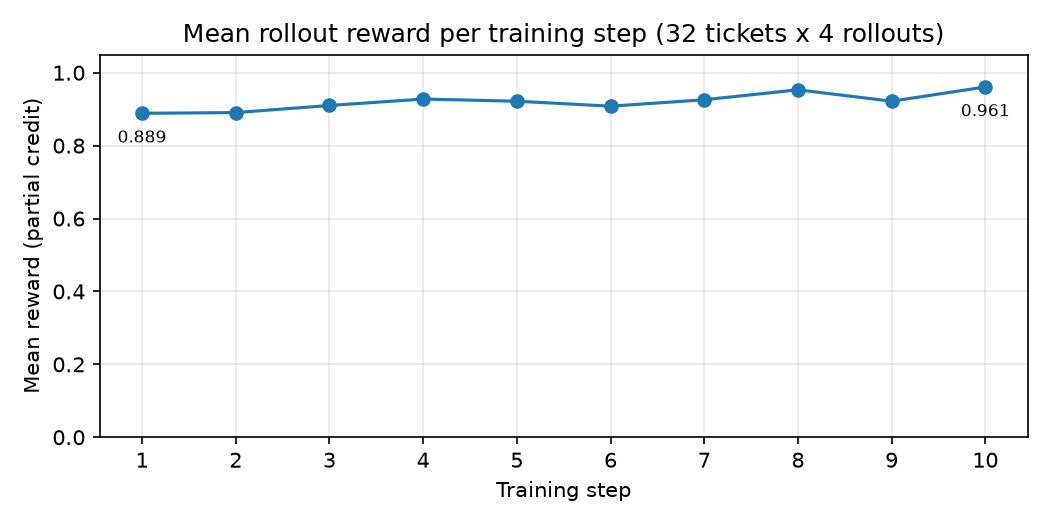
\includegraphics[width=0.82\linewidth]{../figures/training_reward_curve.png}
\captionof{figure}{Mean rollout reward per training step (32 tickets x 4 rollouts per step).}
\end{center}
\begin{center}
\begin{minipage}{\linewidth}\centering
\captionof{table}{Training metrics per step (\texttt{training\_steps.csv}).}
\begin{tabular}{rrrrr}
\toprule
\textbf{Step} & \textbf{Mean reward} & \textbf{Mean turns} & \textbf{Tokens} & \textbf{Trajectories} \\
\midrule
1 & 0.8887 & 6.4844 & 534,113 & 128 \\
2 & 0.8906 & 6.7969 & 571,359 & 128 \\
3 & 0.9102 & 6.8438 & 575,191 & 128 \\
4 & 0.9277 & 6.6328 & 548,452 & 128 \\
5 & 0.9219 & 6.625 & 544,954 & 128 \\
6 & 0.9082 & 6.5 & 533,159 & 128 \\
7 & 0.9258 & 6.6406 & 556,316 & 128 \\
8 & 0.9531 & 7.0234 & 600,379 & 128 \\
9 & 0.9219 & 7 & 593,296 & 128 \\
10 & 0.9609 & 6.5703 & 542,394 & 128 \\
\bottomrule
\end{tabular}
\end{minipage}
\end{center}

\subsection{Held-out evaluation}
\begin{center}
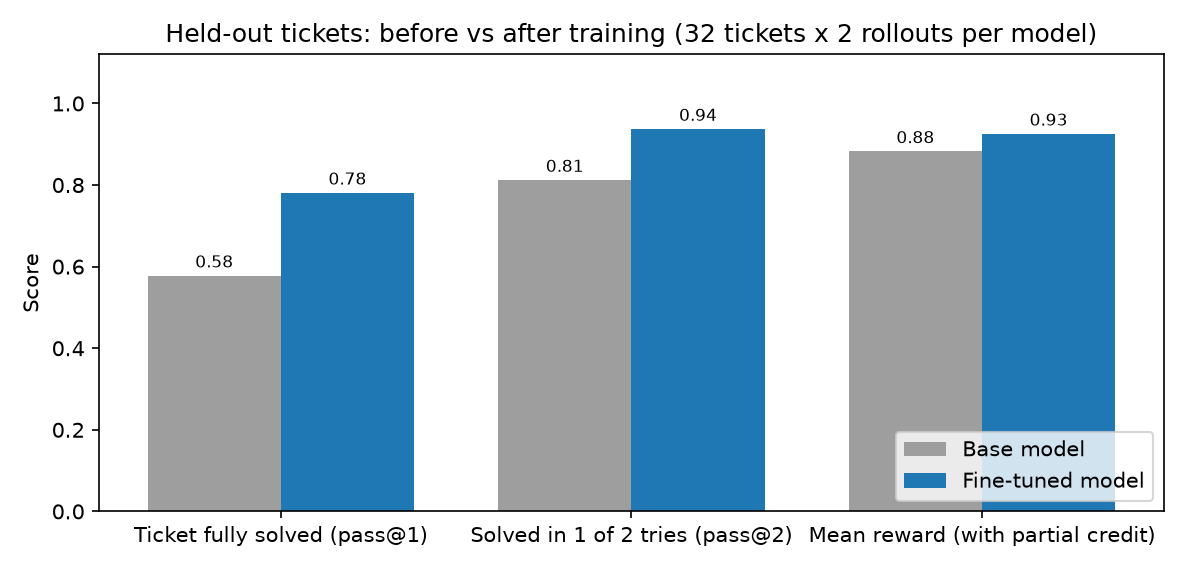
\includegraphics[width=0.82\linewidth]{../figures/evaluation_before_after.png}
\captionof{figure}{Held-out tickets before vs after training (32 tickets x 2 rollouts per model).}
\end{center}
\begin{center}
\begin{minipage}{\linewidth}\centering
\captionof{table}{Held-out evaluation (\texttt{evaluation\_comparison.csv}).}
\begin{tabular}{P{6.4cm}rrr}
\toprule
\textbf{Metric} & \textbf{Base} & \textbf{Fine-tuned} & \textbf{Change} \\
\midrule
Ticket fully solved (pass@1) & 0.5781 & 0.7812 & 0.2031 \\
Solved in 1 of 2 tries (pass@2) & 0.8125 & 0.9375 & 0.125 \\
Mean reward (with partial credit) & 0.8828 & 0.9258 & 0.043 \\
Rollouts fully solved & 37 & 50 & 13 \\
Rollouts not fully solved & 27 & 14 & -13 \\
Model calls per rollout & 6.0938 & 6.4531 & 0.3594 \\
\bottomrule
\end{tabular}
\end{minipage}
\end{center}
\begin{center}
\begin{minipage}{\linewidth}\centering
\captionof{table}{The two baselines (\texttt{baseline\_evaluations.csv}).}
\begin{tabular}{P{6.4cm}rr}
\toprule
\textbf{Metric} & \textbf{First attempt} & \textbf{Baseline of record} \\
\midrule
Ticket fully solved (pass@1) & 0 & 0.5 \\
Solved in 1 of 2 tries (pass@2) & 0 & 0.8438 \\
Mean reward (with partial credit) & 0 & 0.875 \\
Rollouts fully solved & 0 & 32 \\
Rollouts not fully solved & 64 & 32 \\
Model calls per rollout & 2 & 5.8438 \\
\bottomrule
\end{tabular}
\end{minipage}
\end{center}

\subsection{Per held-out ticket}
\begin{center}
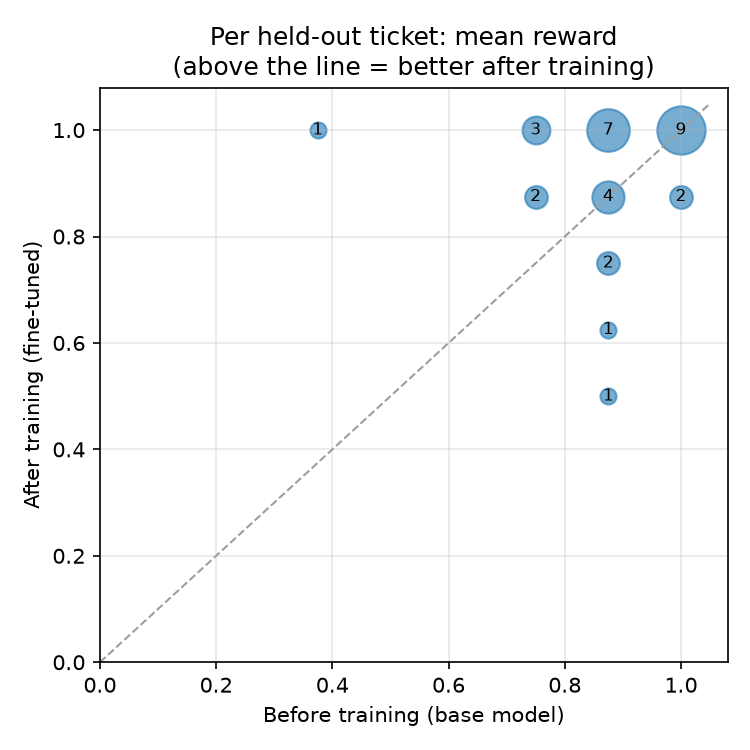
\includegraphics[width=0.82\linewidth]{../figures/per_ticket_before_after.png}
\captionof{figure}{Mean reward per held-out ticket before (x) and after (y) training; point size counts tickets with the same pair.}
\end{center}
{\small
\begin{longtable}{P{5.6cm}llrrl}
\caption{Every held-out ticket (\texttt{per\_ticket\_rewards.csv}).} \\
\toprule
\textbf{Held-out ticket} & \textbf{Before} & \textbf{After} & \textbf{Mean before} & \textbf{Mean after} & \textbf{Change} \\
\midrule
\endfirsthead
\multicolumn{6}{l}{\textit{continued}} \\
\toprule
\textbf{Held-out ticket} & \textbf{Before} & \textbf{After} & \textbf{Mean before} & \textbf{Mean after} & \textbf{Change} \\
\midrule
\endhead
\bottomrule
\endlastfoot
My Wi-Fi works, but websites do not load. & 1.0; 0.75 & 1.0; 0.25 & 0.875 & 0.625 & worse \\
The internet light changed from green to red. & 1.0; 0.75 & 1.0; 1.0 & 0.875 & 1 & improved \\
My service stopped working after a plan change. & 0.75; 0.75 & 1.0; 0.75 & 0.75 & 0.875 & improved \\
Every browser reports that I am offline. & 0.75; 0.75 & 1.0; 1.0 & 0.75 & 1 & improved \\
The router broadcasts Wi-Fi but has no external connection. & 0.75; 1.0 & 0.75; 0.75 & 0.875 & 0.75 & worse \\
The WAN indicator is red after this morning's update. & 0.75; 0.75 & 1.0; 1.0 & 0.75 & 1 & improved \\
All of my smart-home devices lost access at once. & 0.75; 1.0 & 1.0; 0.75 & 0.875 & 0.875 & same \\
Rebooting both modem and router changed nothing. & 1.0; 1.0 & 1.0; 1.0 & 1 & 1 & same \\
Service disappeared after my account details changed. & 1.0; 1.0 & 1.0; 1.0 & 1 & 1 & same \\
My devices connect locally but cannot reach cloud services. & 0.75; 1.0 & 1.0; 1.0 & 0.875 & 1 & improved \\
The router dashboard reports no upstream service. & 1.0; 1.0 & 1.0; 1.0 & 1 & 1 & same \\
Internet access failed after the provider migrated my account. & 1.0; 1.0 & 0.75; 1.0 & 1 & 0.875 & worse \\
The WAN status is red although Wi-Fi strength is excellent. & 1.0; 0.75 & 1.0; 1.0 & 0.875 & 1 & improved \\
Every application times out on every device. & 1.0; 1.0 & 1.0; 1.0 & 1 & 1 & same \\
My connection vanished shortly after a subscription change. & 0.75; 1.0 & 0.75; 0.75 & 0.875 & 0.75 & worse \\
The router is powered and broadcasting but nothing loads. & 1.0; 0.75 & 1.0; 0.0 & 0.875 & 0.5 & worse \\
Phones and computers all say no internet access. & 1.0; 1.0 & 1.0; 1.0 & 1 & 1 & same \\
The external network light is solid red. & 1.0; 1.0 & 1.0; 1.0 & 1 & 1 & same \\
I lost service after customer support modified my account. & 1.0; 1.0 & 1.0; 1.0 & 1 & 1 & same \\
Local network sharing works but the internet does not. & 0.75; 1.0 & 1.0; 0.75 & 0.875 & 0.875 & same \\
The modem status page shows an upstream fault. & 1.0; 0.75 & 1.0; 1.0 & 0.875 & 1 & improved \\
Our connection dropped immediately after a package change. & 0.75; 1.0 & 1.0; 1.0 & 0.875 & 1 & improved \\
Video streaming and websites fail throughout the house. & 1.0; 1.0 & 1.0; 1.0 & 1 & 1 & same \\
The internet indicator turned red without warning. & 0.75; 1.0 & 1.0; 1.0 & 0.875 & 1 & improved \\
Wi-Fi is visible on all devices but none can go online. & 0.75; 0.75 & 1.0; 1.0 & 0.75 & 1 & improved \\
My account was migrated and the connection stopped. & 1.0; 1.0 & 1.0; 0.75 & 1 & 0.875 & worse \\
The router reports connected devices but no internet route. & 0.75; 0.75 & 0.75; 1.0 & 0.75 & 0.875 & improved \\
Restarting the equipment did not clear the red WAN light. & 1.0; 1.0 & 1.0; 1.0 & 1 & 1 & same \\
Our whole home has been offline since the account update. & 0.75; 1.0 & 0.75; 1.0 & 0.875 & 0.875 & same \\
I have full wireless signal and zero internet connectivity. & 0.0; 0.75 & 1.0; 1.0 & 0.375 & 1 & improved \\
The broadband connection is down on every device. & 0.75; 1.0 & 1.0; 1.0 & 0.875 & 1 & improved \\
The router's external link failed after a service change. & 1.0; 0.75 & 0.75; 1.0 & 0.875 & 0.875 & same \\
\end{longtable}
}

\subsection{Live inference}
\begin{center}
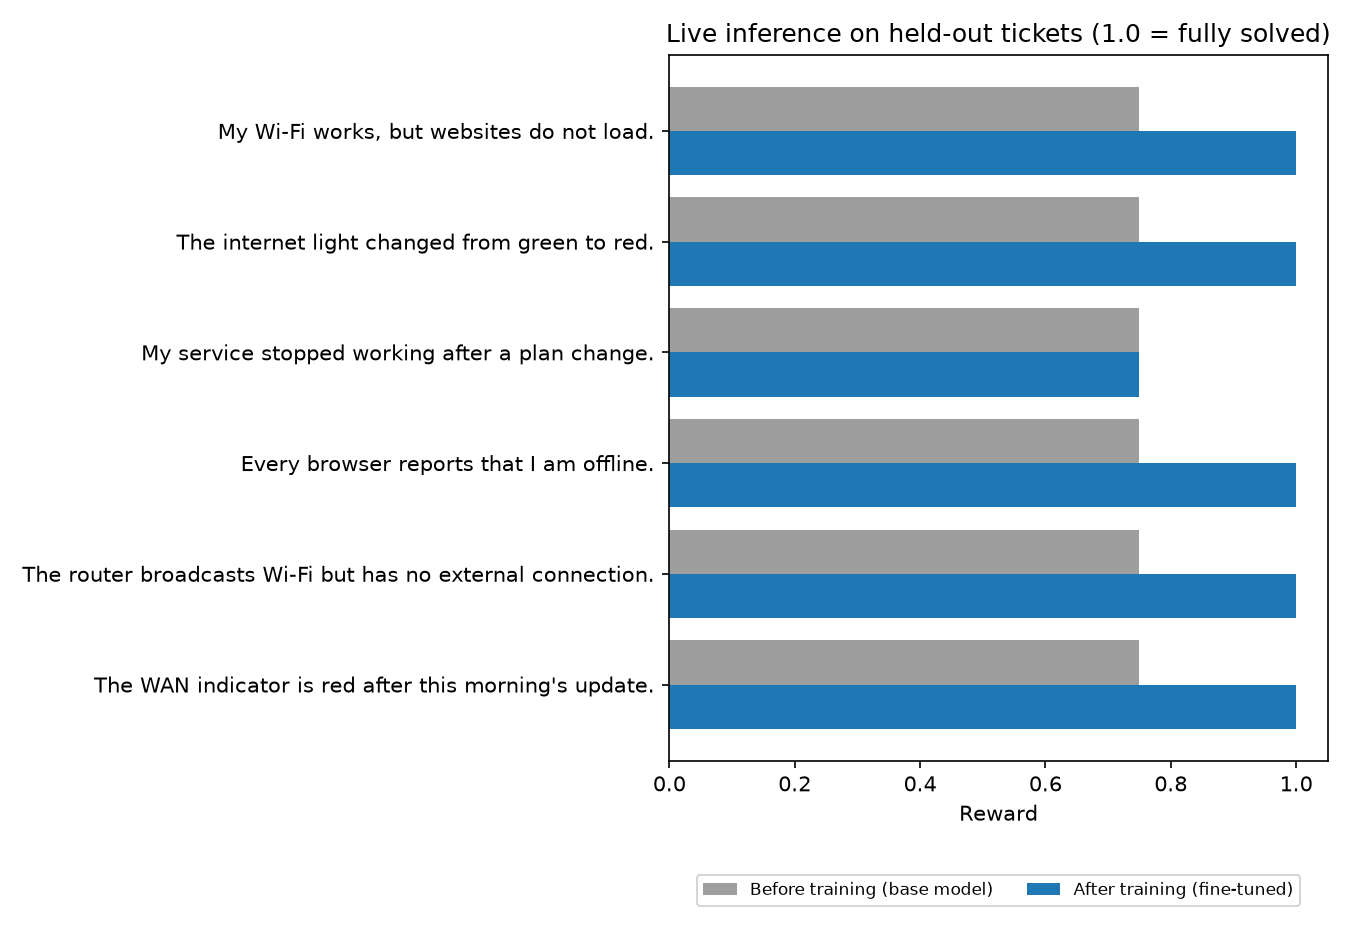
\includegraphics[width=0.82\linewidth]{../figures/live_inference_before_after.png}
\captionof{figure}{Live inference on held-out tickets with the same agent and seed.}
\end{center}
{\small
\begin{center}
\begin{minipage}{\linewidth}\centering
\captionof{table}{Live inference (\texttt{live\_inference.csv}).}
\begin{tabular}{P{3.3cm}rrP{4.8cm}P{4.8cm}}
\toprule
\textbf{Ticket} & \textbf{Before} & \textbf{After} & \textbf{Before: actions} & \textbf{After: actions} \\
\midrule
My Wi-Fi works, but websites do not load. & 0.75 & 1 & restart\_router > check\_outage > inspect\_router\_lights > check\_account\_config & check\_outage > inspect\_router\_lights > check\_account\_config > apply\_config\_fix \\
The internet light changed from green to red. & 0.75 & 1 & restart\_router > check\_outage > inspect\_router\_lights > check\_account\_config & check\_outage > inspect\_router\_lights > check\_account\_config > apply\_config\_fix \\
My service stopped working after a plan change. & 0.75 & 0.75 & restart\_router > check\_outage > inspect\_router\_lights > check\_account\_config & restart\_router > check\_outage > inspect\_router\_lights > check\_account\_config \\
Every browser reports that I am offline. & 0.75 & 1 & restart\_router > check\_outage > inspect\_router\_lights > check\_account\_config & check\_outage > inspect\_router\_lights > check\_account\_config > apply\_config\_fix \\
The router broadcasts Wi-Fi but has no external connection. & 0.75 & 1 & restart\_router > check\_outage > inspect\_router\_lights > check\_account\_config & check\_outage > inspect\_router\_lights > check\_account\_config > apply\_config\_fix \\
The WAN indicator is red after this morning's update. & 0.75 & 1 & restart\_router > check\_outage > inspect\_router\_lights > check\_account\_config & check\_outage > inspect\_router\_lights > check\_account\_config > apply\_config\_fix \\
\bottomrule
\end{tabular}
\end{minipage}
\end{center}
}

\subsection{Run of record}
{\small
\begin{longtable}{P{3.2cm}P{3.6cm}P{1.8cm}P{6.6cm}}
\caption{Run of record (\texttt{run\_of\_record.csv}).} \\
\toprule
\textbf{Stage} & \textbf{Identifier} & \textbf{Status} & \textbf{Detail} \\
\midrule
\endfirsthead
\multicolumn{4}{l}{\textit{continued}} \\
\toprule
\textbf{Stage} & \textbf{Identifier} & \textbf{Status} & \textbf{Detail} \\
\midrule
\endhead
\bottomrule
\endlastfoot
Base evaluation (first attempt) & 59n0c9w40lyx & Succeeded & pass@1 0, mean reward 0 \\
Base evaluation & 7kz12i8e43ip & Succeeded & pass@1 0.5, mean reward 0.875 \\
Training (rejected attempt) & openai-reasoning-gpt-oss-20b-mtrl-20261002040240 & Failed & ClientError: Training data has 32 prompts but global\_batch\_size is 32. The number of prompts must be greater than the batch size. \\
Training & openai-reasoning-gpt-oss-20b-mtrl-20261002040558 & Completed & 10/10 steps in 19.2 min; model package arn:aws:sagemaker:us-west-2:384887233198:model-package/openai-reasoning-gpt-oss-20b-mtrl-mpg/1 \\
Comparison evaluation & 8hvze02od4o0 & Succeeded & pass@1 base 0.578125 -> fine-tuned 0.78125 \\
SageMaker endpoint & mtrl-support-demo & Deleted & Unable to provision requested ML compute capacity due to InsufficientInstanceCapacity error; billed \$0.0 \\
Bedrock import & mtrl-support-import-20261002051532 & Completed & imported model arn:aws:bedrock:us-east-1:384887233198:imported-model/ffakmfmpoqbi \\
Live inference & seed 2026 & Recorded & fully solved: before 0/6, after 5/6 \\
\end{longtable}
}

\subsection{Provenance: what actually ran}
Every rollout of the baseline of record, the training job, and the comparison was served by one AgentCore runtime version, last updated before all three jobs started. The Bedrock import read the us-east-1 copy of the trained package's merged weights. Both are recorded by scripts/11b\_snapshot\_provenance.py and checked by the invariants:
\begin{center}
\begin{minipage}{\linewidth}\centering
\begin{tabular}{P{3.4cm}P{12cm}}
\toprule
\textbf{Record} & \textbf{Value} \\
\midrule
AgentCore runtime & version 7, last updated 2026-10-01 23:13:23 UTC \\
Container image & \texttt{\scriptsize sha256:af5cb1b29526c440f2cb77f4f62f81980b9291a7a3c9d349ca280a0fd45c603f} \\
Base image & \texttt{\scriptsize python:3.12-slim}\newline \texttt{\scriptsize sha256:f77ac9e44ae96ef2c90b8053ea08c31f8be030f824196b0ae4db6d462c84e51f} \\
CodeBuild build & \texttt{\scriptsize b599bfe5-116b-452d-ac78-eb3b6a039d75} \\
Source bundle & \texttt{artifacts/agent\_deployed\_source.zip}, SHA-256 \texttt{\scriptsize c3507c9bf606754cd18cca659ffce779cfb48f020b4bb945f12d0247ae284430} \\
Import read from & \nolinkurl{s3://sagemaker-mtrl-demo-384887233198-us-east-1/imported-models/mtrl-support-gpt-oss-20b-ft/} \\
\bottomrule
\end{tabular}
\end{minipage}
\end{center}
\begin{center}
\begin{minipage}{\linewidth}\centering
\captionof{table}{The agent's deployed source bundle against the repository's \texttt{agent/}.}
\begin{tabular}{P{4.4cm}lP{8.2cm}}
\toprule
\textbf{Deployed file} & \textbf{SHA-256 (start)} & \textbf{Repository today} \\
\midrule
\texttt{Dockerfile} & \texttt{8f6841277ac06dd6} & identical \\
\texttt{app.py} & \texttt{c08bca8ab9dc63c2} & refactored after the deploy (run\_episode); same system prompt \\
\texttt{environment.py} & \texttt{b19daf0ffc39792f} & identical \\
\texttt{pyproject.toml} & \texttt{1fac4fd7a60a9bc5} & ranges when built; now exact pins \\
\texttt{requirements.txt} & \texttt{09c3b4f36fb2253a} & ranges when built; now exact pins, equal to the image's versions \\
\texttt{rollout\_driver.py} & \texttt{a7c415a6829d2050} & identical \\
\texttt{test\_app.py} & \texttt{f930004923547b2a} & test file; not used at runtime \\
\texttt{test\_environment.py} & \texttt{c22cc1c562e5df48} & identical \\
\texttt{test\_rollout\_driver.py} & \texttt{1b22e6738281e9ca} & identical \\
\bottomrule
\end{tabular}
\end{minipage}
\end{center}
{\small
\begin{center}
\begin{minipage}{\linewidth}\centering
\captionof{table}{The imported model's files against the trained package's merged weights.}
\begin{tabular}{P{5.6cm}rrl}
\toprule
\textbf{File} & \textbf{Package bytes} & \textbf{Copy bytes} & \textbf{Verdict} \\
\midrule
\texttt{\_\_model\_info\_\_.json} & 190 & -- & not copied \\
\texttt{\_\_script\_info\_\_.json} & 161 & -- & not copied \\
\texttt{chat\_template.jinja} & 13,653 & 13,653 & identical \\
\texttt{chat\_template.json} & 14,385 & 14,385 & identical \\
\texttt{config.json} & 1,588 & 1,588 & identical \\
\texttt{generation\_config.json} & 165 & 176 & changed on purpose \\
\texttt{inference.py} & 0 & -- & not copied \\
\texttt{model-00000-of-00002.safetensors} & 16,487,374,440 & 16,487,374,440 & same size \\
\texttt{model-00001-of-00002.safetensors} & 16,493,804,168 & 16,493,804,168 & same size \\
\texttt{model-00002-of-00002.safetensors} & 8,848,382,808 & 8,848,382,808 & same size \\
\texttt{model.safetensors.index.json} & 33,597 & 33,597 & identical \\
\texttt{o200k\_base.tiktoken} & 3,613,922 & 3,613,922 & identical \\
\texttt{special\_tokens\_map.json} & 98 & 98 & identical \\
\texttt{tokenizer.json} & 27,868,174 & 27,868,174 & same size \\
\texttt{tokenizer\_config.json} & 4,200 & 18,582 & changed on purpose \\
\texttt{version} & 5 & -- & not copied \\
\bottomrule
\end{tabular}
\end{minipage}
\end{center}
}

\section{Invariant Checks}
\texttt{scripts/14\_verify\_invariants.py} re-checks, offline and from the files on disk, every property the
results depend on, and prints a PASS/FAIL line for each. All 19 pass on the evidence in this repository.
\begin{enumerate}[leftmargin=*,itemsep=1pt]
\item settings in aws/config.py match the documented protocol
\item datasets: sizes, uniqueness, held-out disjoint
\item datasets unchanged since the run of record
\item S3 datasets equal the CSVs and predate the jobs
\item agent that ran matches the repository (code, prompt, packages)
\item training job ran the documented protocol
\item base model version matches the run of record
\item training metrics recorded for every step
\item baseline had a learning signal
\item comparison evaluation succeeded, 32 x 2 per model
\item recorded traces recompute the evaluation metrics
\item deployed model traces back to the trained package
\item live inference: first held-out tickets, documented seed, no errors
\item no endpoint left running
\item cost accounting complete, recomputable, within the cap
\item no signed links in evidence, notebooks, reports, or logs
\item environment matches the exact pins
\item notebooks parse and ran without exceptions
\item report tables equal a rebuild from evidence; figures present
\end{enumerate}

\section{Held-out Discipline and Provenance Controls}
The 32 held-out tickets are fixed before any training and never enter it. The two prompt files
share no prompt (invariant~2), and both match the run of record by SHA-256
(invariant~3). Training reads only the training tickets. The baseline, the comparison, and
the live inference read only held-out tickets. The live inference uses the first 6 held-out
tickets in file order with the documented seed (invariant~13). Both models in the comparison are
evaluated by one pipeline, on the same tickets, through the same agent and serving stack, so the comparison
isolates the effect of training.

Provenance closes the remaining gap between the repository and what ran:
\begin{itemize}[leftmargin=*]
\item \textbf{Agent.} The AgentCore runtime that served every rollout went live before all three jobs
started, and was built from the saved source bundle. That bundle's environment, rollout driver, Dockerfile,
and system prompt match the repository (invariant~5).
\item \textbf{Datasets.} The S3 datasets the jobs read equal the CSVs, and were written before the jobs
(invariant~4).
\item \textbf{Imported model.} It was built from the trained package's merged weights, changing only the
two files the Bedrock documentation requires (invariant~12).
\end{itemize}

\appendix
\section{Software Engineering Practices}
The study code is treated as software, not throwaway scripts. Each practice below names the concrete
mechanism in the codebase.
\begin{itemize}[leftmargin=*]
\item \textbf{Separation of concerns.} The \texttt{aws} package is organised by stage: \texttt{setup/},
\texttt{rl/}, \texttt{deploy/}, \texttt{costs/}, \texttt{records/}, and \texttt{reporting/}, with
\texttt{workflow.py} as the single facade. The numbered scripts are thin entry points, and \texttt{agent/} is
kept identical to what ran.
\item \textbf{DRY (single source of truth).} Settings and project paths live once in \texttt{aws/config.py}.
One table builder serves both script 12 and the invariants. The notebook and the scripts call the same
modules, and the notebook is generated by \texttt{scripts/dev/build\_notebook.py} and checked against it.
\item \textbf{Immutable values and write-once evidence.} Settings and the protocol are frozen dataclasses.
The evidence of record is never overwritten: a later live run is saved beside it, and a failed job is
archived before it is replaced.
\item \textbf{Fail-fast errors.} A missing evidence file raises \texttt{FileNotFoundError} naming the script
that produces it. A wrong confirmation phrase raises \texttt{PermissionError}. The budget guard refuses before
any billable work.
\item \textbf{Cost safety.} Every billable step needs an exact confirmation phrase, passes the budget guard,
and re-attaches to a recorded job instead of resubmitting it. A watchdog deletes the endpoint at its
deadline.
\item \textbf{Reproducibility hygiene.} The project uses only project-relative paths, and the environments
are pinned and locked. \texttt{run\_commands.csv} is ordered, \texttt{study\_metadata.json} is
machine-readable, and evidence is written atomically with signed links redacted. Logs are scrubbed of links
and of the home-folder path.
\item \textbf{Verify before asserting.} The invariants recompute the metrics from the recorded conversations,
the costs from token usage and rates, and the tables from the evidence. This sheet is built only when all of
them pass.
\item \textbf{Tests and style.} 302 unit tests (\texttt{tests/} mirrors \texttt{aws/};
\texttt{agent/} has its own) run with \texttt{python -m pytest} and need no AWS access. The code has
Google-style docstrings and type hints throughout, and passes \texttt{ruff}.
\end{itemize}

\end{document}
